\ifdefined\pres
\documentclass{beamer}
\else
\documentclass{paper}
\fi
\usepackage[utf8]{inputenc}
\usepackage[T2A,T1]{fontenc}
\usepackage[english, russian]{babel}
\usepackage{etoolbox}
\usepackage{amssymb}
\usepackage{listings}
\usetheme{Pittsburgh}

\selectlanguage{russian}
\newcommand{\define}[2]{{\bf #1} --- #2.\vspace{1em}}
\newcommand{\longdef}[1]{{\textbf{\underline{Опр:}} #1}}
\newcommand{\set}[1]{{\lbrace #1 \rbrace}}

\newtoggle{mynotes}

\ifdefined\pres
\togglefalse{mynotes}
\else
\toggletrue{mynotes}
\fi

\iftoggle{mynotes}{
  \newcommand{\mynote}[1]{mynote: #1}
}{
  \newcommand{\mynote}[1]{}
}

\title{Симметричная криптография. Потоковые шифры}
\institute{ВГУ}
\date{2014}
\begin{document}

\frame{\titlepage}

\begin{frame}
  \frametitle{Классификация криптографических алгоритмов}

  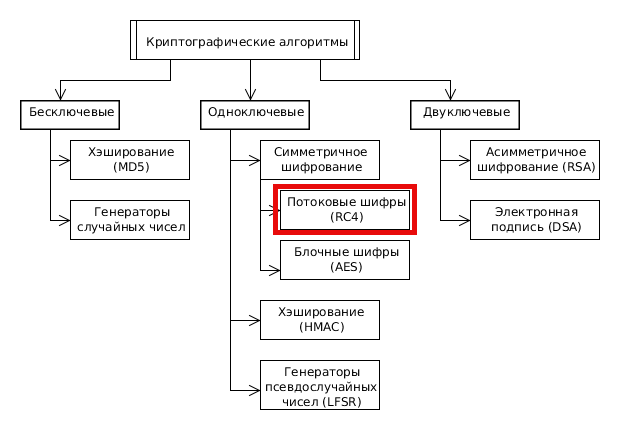
\includegraphics[width=\linewidth]{./imgs/CA_classification_stream.png}

\end{frame}

\begin{frame}
  \frametitle{Свойства операции xor}

  \begin{itemize}
    \item{$a \oplus (b \oplus c) = (a \oplus b) \oplus c$}
    \item{$a \oplus a = 0$}
    \item{$a \oplus b = c \Rightarrow a \oplus c = b$}
  \end{itemize}
\end{frame}


\begin{frame}
  \frametitle{Симметричная криптография}

  \begin{block}{Протокол передачи зашифрованного сообщения}
  \begin{enumerate}
    \item{Алиса и Боб выбирают систему шифрования}
    \item{Алиса и Боб выбирают ключ}
    \item{Алиса шифрует открытый текст с использованием алгоритма шифрования и ключа}
    \item{Алиса посылает шифрованное сообщение Бобу}
    \item{Боб дешифрует шифротекст с использованием того же алгоритма и ключа}
  \end{enumerate}
  \end{block}
\end{frame}


\begin{frame}
  \frametitle{Определение шифра}

  \longdef{Шифром, определенным на $(K,M,C)$, называется пара <<эффективно>> вычислимых алгоритмов $(E,D)$, где \newline
    \[E: K \times M \longrightarrow C \]
    \[D: K \times C \longrightarrow M, \]
    \[s.t. ~ \forall m \in M, k \in K: D(k, E(k,m)) = m \]
  }

  \mynote{
  $E$ часто является рандомизированным алгоритмом, т.е. использует
  некоторую случайную информацию во время своей работы. То есть, для одних
  и тех же значений  $k$ и $m$ результат $c$ может отличаться.
  Алгоритм же $D$ всегда детерминирванный. Для одних и тех же значений
  входных параметров $c$ и $k$ результат одинаков.
  }
\end{frame}


\begin{frame}
  \frametitle{Шифрование с помощью одноразовых блокнотов (one time pad)}

  \begin{itemize}
    \itemsep 2em
    \item{Множества, на которых определен шифр: \newline
      $M=C=\set{0,1}^{n}, K=\set{0,1}^{n}$}
    \item{Функция шифрования: \newline
      $E(k,m)=k \oplus m$}
    \item{Функция дешифрования: \newline
      $D(k,c)=k \oplus c$}

    \mynote{Пример работы алгоритма. Проверка равенства $D(k, E(k,m)) = m$}
    \mynote{Необходимо заметить, что алгоритм выполняется над потоком бит потенциально бесконечной длины}
    \mynote{По известному открытому сообщению и шифротексту можно легко найти
    часть ключа. Но эту часть ключа можно использовать только для расшифрования
    уже извесного открытого текста}
  \end{itemize}

\end{frame}


\begin{frame}
  \frametitle{Шифрование с помощью одноразовых блокнотов (one time pad)}

  \begin{block} {Преимущества}
    \begin{itemize}
      \item{Высокая скорость шифрования и дешифрования}
    \end{itemize}
  \end{block}

  \begin{block} {Недостатки}
    \begin{itemize}
      \item{Размер ключа равен размеру шифруемого текста}
    \end{itemize}
  \end{block}

  \vspace{2 em}
  Насколько хорош алгоритм с точки зрения безопасности?

\end{frame}


\begin{frame}
  \frametitle{Совершенная безопасность шифра}

  \textbf{Основная идея:} По известному шифротексту невозможно извлечь какую-либо информацию об открытом тексте.
  \mynote{Здесь предполагается, что злоумышленник может использовать только атаку
  на шифротекст, то есть по известному шифротексту пытаться узнать ключ или
  содержание открытого сообщения}
  \vspace{2em}

  \longdef{Шифр $(E,D)$, определенный на $(K,M,C)$ имеет совершенную безопасность, если \newline
    $\forall m_{0},m_{1} \in M:  |m_{0}| = |m_{1}|$ и $\forall c \in C$
      \begin{center} $Pr[E(k,m_{0}) = c] = Pr[E(k,m_{1}) = c]$, \end{center}
      где $k \stackrel{R}{\longleftarrow}K$}

  \mynote{Пояснение: Если известно некоторое зашифрованное сообщение $c$, то
    вероятности того, что зашифровано сообщение $m_{0}$ или $m_{1}$ равны. То
    есть по зашифрованному сообщению невозможно определить какое из сообщений
    более вероятно было зашифровано}
  \mynote{Шеннон теоретически показал, что совершенная безопасность возможна}
  \mynote{Informally,if you intercept a cipher-text from a perfectly secure
    encryption system, you can find a key that causes that cipher-text to
    decrypt to any message you want (of the correct length). So without
    knowing which key the author actually picked, you never learn anything
    about the message. This holds even if you try every possible key (because
    all keys decrypt the cipher-text to a possibly valid message)}

\end{frame}


\begin{frame}
  \frametitle{Совершенная безопасность шифра}

  \begin{itemize}
    \item{Шифрование с помощью одноразовых блокнотов имеет совершенную безопасность}
    \item{Для того, чтобы шифр имел совершенную безопасность, необходимо, чтобы $|K| \ge |M|$, поэтому использование
          шифров с совершенной безопасностью на практике затруднено}
  \end{itemize}
\end{frame}


\begin{frame}
  \frametitle{Потоковые шифры}

  \textbf{Основная идея:} Замена "случайного" ключа на "псевдослучайный" ключ.
  \vspace{1em}

  Для этого используются генераторы псевдослучайных чисел (ГПЧ).
  \vspace{1em}

  \[G:\set{0,1}^{s} \mapsto \set{0,1}^{n}, n \gg s\]

  \mynote{Требования к генератору: 
    1. Должен существовать детерминистический алгоритм, который может быть эффективно выполнен для реализации генератора.
       Единственный элемент, который остается случайным - это seed.
    2. Выходная строка должна выглядеть случайно
    Открытый вопрос: что значит выглядеть случайно?
  }

\end{frame}


\begin{frame}
  \frametitle{Потоковые шифры}

  Так как ГПЧ может генерировать псевдослучайные строки большой длины, то можно создать шифр,
  аналогичный шифру с одноразовыми блокнотами. Главное отличие - длина ключа фиксирована и много меньше, чем длина
  сообщения.

  \begin{itemize}
    \itemsep 2em
    \item{Функция шифрования: \newline
      $E(k,m)=m \oplus G(k)$}
    \item{Функция дешифрования: \newline
      $D(k,c)=c \oplus G(k)$}

    \mynote{Показать на рисунке как из маленького ключа получается длинная последовательность}
    \mynote{Открытый вопрос: насколько такой шифр безопасен? Необходимо новое определение безопасности}
  \end{itemize}

\end{frame}


\begin{frame}
  \frametitle{Потоковые шифры}

  \mynote{Главным уязвимым звеном в потоковых шифрах становится ГСЧ}

  Необходимое условие безопасности поточного шифра - непредсказуемость ГСЧ.

  \vspace{1em}

  Если ГСЧ предсказуем, то

  \[\exists i: G(k)|_{1 \ldots i} \stackrel{alg}{\longrightarrow} G(k)|_{i+1 \ldots n}\]

  \mynote{Предсказуемость ГСЧ может полностью свести безопасность потокового шифра на нет.
    Пример - протокол SMTP. Так как любое письмо начинается с FROM:, то злоумышленник может определить первые 5
    байт, сгенерированных ГСЧ и предсказать последующие биты ГСЧ}

  \mynote{Многие реализации ГСЧ, которые поставляются в стандартных библиотеках, на самом деле легко предсказуемы.
    Например, реализация функции random() в библиотеке glibc. Kerberos v.4 использовало эту функцию, что привело к её взлому.}

\end{frame}


\begin{frame}
  \frametitle{Предсказуемость ГСЧ}

  \longdef{ГСЧ $G:K \longrightarrow \set{0,1}^{r}$ называется предсказуемым, если существует
   эффективно вычислимый алгоритм $A$ и $\exists 1 \le i \le n-1$ такое, что
    \begin{displaymath}
      {Pr_{k \stackrel{R}{\longleftarrow} K}[A(G(k))|_{1 \ldots i} = G(k)|_{i+1}] \ge 1/2 + \varepsilon}
    \end{displaymath}
  }

\end{frame}


\begin{frame}
  \frametitle{Предсказуемые ГСЧ}

  \begin{block}{Линейный конгруэнтный метод}
    \begin{itemize}
      \item{Три параметра: a, b, p}
      \item{$r[0] = seed$}
      \item{$r[i] = (a*r[i-1]+b)~mod~p$}
      \item{Используется в чистом виде или с некоторыми модификациями во многих реализациях стандартных языковых библиотек}
    \end{itemize}
  \end{block}

\end{frame}


\begin{frame}
  \frametitle{Потоковые шифры. Атаки}

  \begin{block}{Повторное использование ключа в шифровании одноразовыми блокнотами}
    \begin{itemize}
      \item{Ключ для поточного шифра не должен использоваться больше одного раза
        \[ c_{1} \leftarrow m_{1} \oplus PRG(k) \]
        \[ c_{2} \leftarrow m_{2} \oplus PRG(k) \]
        \[ c_{1} \oplus c_{2} =  m_{1} \oplus m_{2} \]
      }
      \item{Существующая избыточность человеческого языка и ASCII-кодирования позволяет восстановить открытый текст}
      \item{Примеры повторного использования ключа: проект ``Венона``, MS-PPTP, WEP}
      \item{Невозможность использования потоковых шифров в некоторых областях (шифрование данных на диске)}
    \end{itemize}
  \end{block}

\end{frame}


\begin{frame}
  \frametitle{Потоковые шифры. Атаки}

  \begin{block}{Невозможность проверки целостности}
    Злоумышленник может изменить зашифрованное сообщение предсказуемым образом:
      \[ c_{Alice} = m \oplus k \]
      \[ c_{Mallory} = c_{Alice} \oplus p \]
      \[ m_{Bob} = c_{Mallory} \oplus k = m \oplus p \]
  \end{block}

\end{frame}


\begin{frame}
  \frametitle{Потоковые шифры. Примеры}

  \begin{itemize}
    \item{RC4}
    \item{Шифры, использующие регистр сдвига с линейной обратной связью (LFSR)}
    \item{Семейство шифров eStream}
  \end{itemize}

\end{frame}

\begin{frame}
  \frametitle{Шифр RC4}

  \begin{itemize}
    \item{$c_{i} = m_{i} \oplus k_{i}$}
  \end{itemize}

  \begin{block}{Входные параметры:}
    \begin{itemize}
      \item{Ключ размером L бит ($40 \le L \le 2048$)}
      \item{$n$ - размер слова для алгоритма}
    \end{itemize}
  \end{block}

  \begin{block}{Внутреннее состояние:}
    \begin{itemize}
      \item{Массив размеров $2^n$ (S-блок)}
      \item{Значения счетчиков $i$,$j$}
    \end{itemize}
  \end{block}
\end{frame}

\begin{frame}
  \frametitle{Шифр RC4}

  \begin{block}{2 стадии генерации ключевого потока}
    \begin{itemize}
      \item{Инициализация S-блока}
      \item{Генерация псевдослучайного слова $K$}
    \end{itemize}
  \end{block}
\end{frame}

\begin{frame}[fragile]
  \frametitle{Шифр RC4}

  \begin{block}{Инициализация S-блока ($n = 8$)}
    \lstset{language=Pascal}
    \begin{lstlisting}[frame=single]
    for i := 0 to 255
        S[i] := i
    end
    j := 0
    for i := 0 to 255
        j := (j + S[i] + Key[i mod L]) mod 256
        swap S[i] and S[j]
    end
    \end{lstlisting}
  \end{block}
\end{frame}

\begin{frame}[fragile]
  \frametitle{Шифр RC4}

  \begin{block}{Генерация псевдослучайного слова $K$}
    \lstset{language=Pascal}
    \begin{lstlisting}[frame=single]
      i := 0
      j := 0
      while (generation cycle):
          i := (i + 1) mod 256
          j := (j + S[i]) mod 256
          swap S[i] and S[j]
          t := (S[i] + S[j]) mod 256
          K := S[t] //generated one word for K
      end
    \end{lstlisting}
  \end{block}
\end{frame}

\begin{frame}
  \frametitle{Шифр RC4}

  \begin{block}{Преимущества}
    \begin{itemize}
      \item{Переменный размер ключа}
      \item{Высокая скорость работы}
    \end{itemize}
  \end{block}

  Применяется в протоколах TLS/SSL, WEP, WPA.
\end{frame}

\end{document}
